\documentclass[border=6pt]{standalone}
\usepackage{amsmath}
\usepackage{tikz}
\usetikzlibrary{positioning, arrows.meta, fit, backgrounds, calc}
\tikzset{stage/.style={draw, rounded corners, align=center, font=\small, minimum height=1.0cm, minimum width=2.6cm, thick},
layer/.style={draw, dashed, rounded corners, inner sep=10pt},
node_t/.style={draw, circle, align=center, font=\scriptsize, minimum size=1.0cm, thick},
flow/.style={-{Stealth[length=2.5mm]}, thick},
edge_t/.style={-{Stealth[length=2mm]}, font=\scriptsize}}
\begin{document}
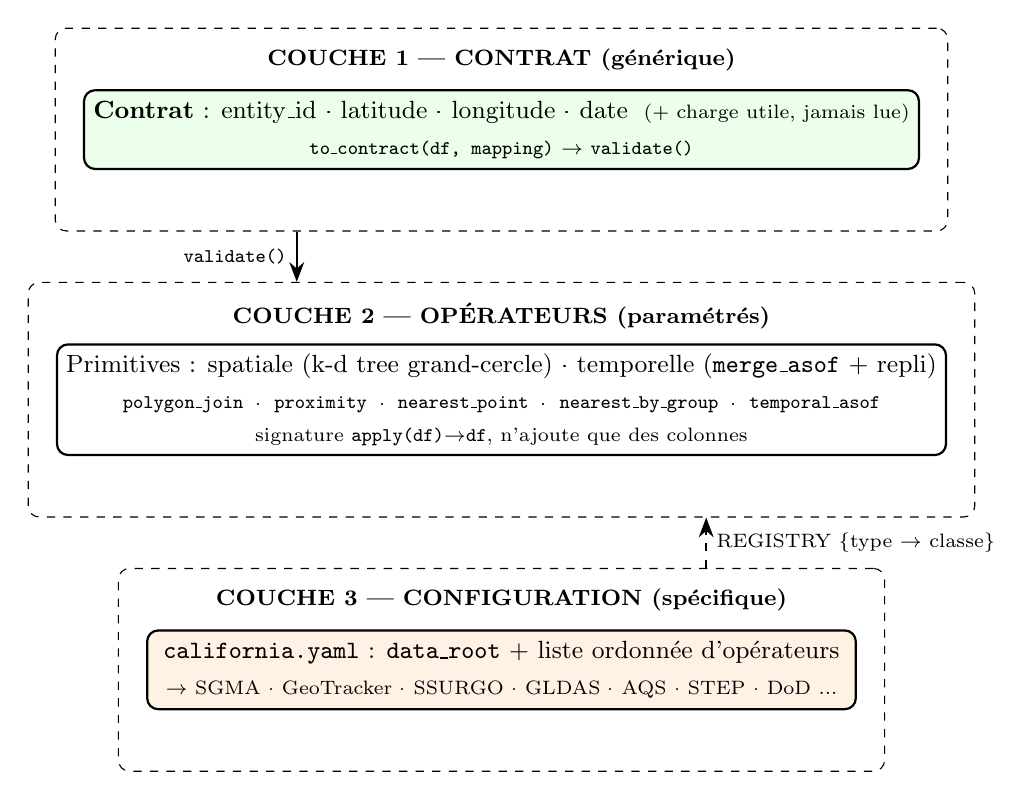
\begin{tikzpicture}[node distance=0.5cm]
  % Couche 1
  \node[stage, fill=green!8, minimum width=9cm] (c1)
    {\textbf{Contrat} : entity\_id · latitude · longitude · date \;{\scriptsize(+ charge utile, jamais lue)}\\[2pt]
     {\scriptsize \texttt{to\_contract(df, mapping)} $\rightarrow$ \texttt{validate()}}};
  \node[layer, fit=(c1), inner ysep=22pt] (l1) {};
  \node[font=\footnotesize\bfseries, anchor=north] at ([yshift=-4pt]l1.north) {COUCHE 1 — CONTRAT (générique)};
  % Couche 2
  \node[stage, below=2.2cm of c1, minimum width=9cm] (ops)
    {Primitives : spatiale (k-d tree grand-cercle) · temporelle (\texttt{merge\_asof} + repli)\\[2pt]
     {\scriptsize \texttt{polygon\_join · proximity · nearest\_point · nearest\_by\_group · temporal\_asof}}\\[1pt]
     {\scriptsize signature \texttt{apply(df)$\to$df}, n'ajoute que des colonnes}};
  \node[layer, fit=(ops), inner ysep=22pt] (l2) {};
  \node[font=\footnotesize\bfseries, anchor=north] at ([yshift=-4pt]l2.north) {COUCHE 2 — OPÉRATEURS (paramétrés)};
  % Couche 3
  \node[stage, fill=orange!10, below=2.2cm of ops, minimum width=9cm] (cfg)
    {\texttt{california.yaml} : \texttt{data\_root} + liste ordonnée d'opérateurs\\[2pt]
     {\scriptsize $\rightarrow$ SGMA · GeoTracker · SSURGO · GLDAS · AQS · STEP · DoD ...}};
  \node[layer, fit=(cfg), inner ysep=22pt] (l3) {};
  \node[font=\footnotesize\bfseries, anchor=north] at ([yshift=-4pt]l3.north) {COUCHE 3 — CONFIGURATION (spécifique)};
  \draw[flow] ([xshift=-2.6cm]l1.south) -- node[left, font=\scriptsize]{\texttt{validate()}} ([xshift=-2.6cm]l2.north);
  \draw[flow, dashed] ([xshift=2.6cm]l3.north) -- node[right, font=\scriptsize]{REGISTRY \{type $\to$ classe\}} ([xshift=2.6cm]l2.south);
\end{tikzpicture}

\end{document}
